\chapter{Summary and Reflections}

\section{Team Members and the Division of Labor}

The implementation-phase allocation used in WR2 preparation is summarised below. It updates the earlier WR1 proposal roles and reflects the work packages needed to turn the concept into a working prototype and report pack.

\begin{itemize}
\item Guangjun HU (20511787): WR2 integration, requirements validation, appendix consolidation, and document traceability.
\item Hongshuo HU (20808603): Unity architecture, scene wiring, core battle systems, and runtime integration.
\item Cheng YE (20513323): UML and figure refinement, prototype presentation material, and supporting chapter drafting.
\item Zehan CHEN (20807750): validation records, testing and meeting templates, and supporting documentation/website tasks.
\end{itemize}

\section{Completed Process}

By the end of this WR2 cycle, the project has moved from a proposal-level concept to a working prototype snapshot. Building on the WR1 requirement baseline, the team produced a constrained architecture definition, implemented the first-pass gameplay modules, captured prototype screenshots, updated the runtime architecture to match the current code, and aligned the report with the current prototype evidence. During closeout, the team also corrected a battle-end accuracy gap by adding battle-end termination and textual outcome feedback, then backed that fix with a small EditMode test suite around the turn manager.

This reporting cycle also exposed a process gap: several implementation records were not yet archived in a reusable structure. WR2 therefore introduces a small project-record set covering meeting notes, process evidence notes, decision logs, validation notes, and testing records. The cleaned GitHub repository now also shows the current closeout workflow through merged document and code pull requests. These records are lightweight so the team can continue using them in WR3 and the final report.

\begin{figure}[H]
\centering
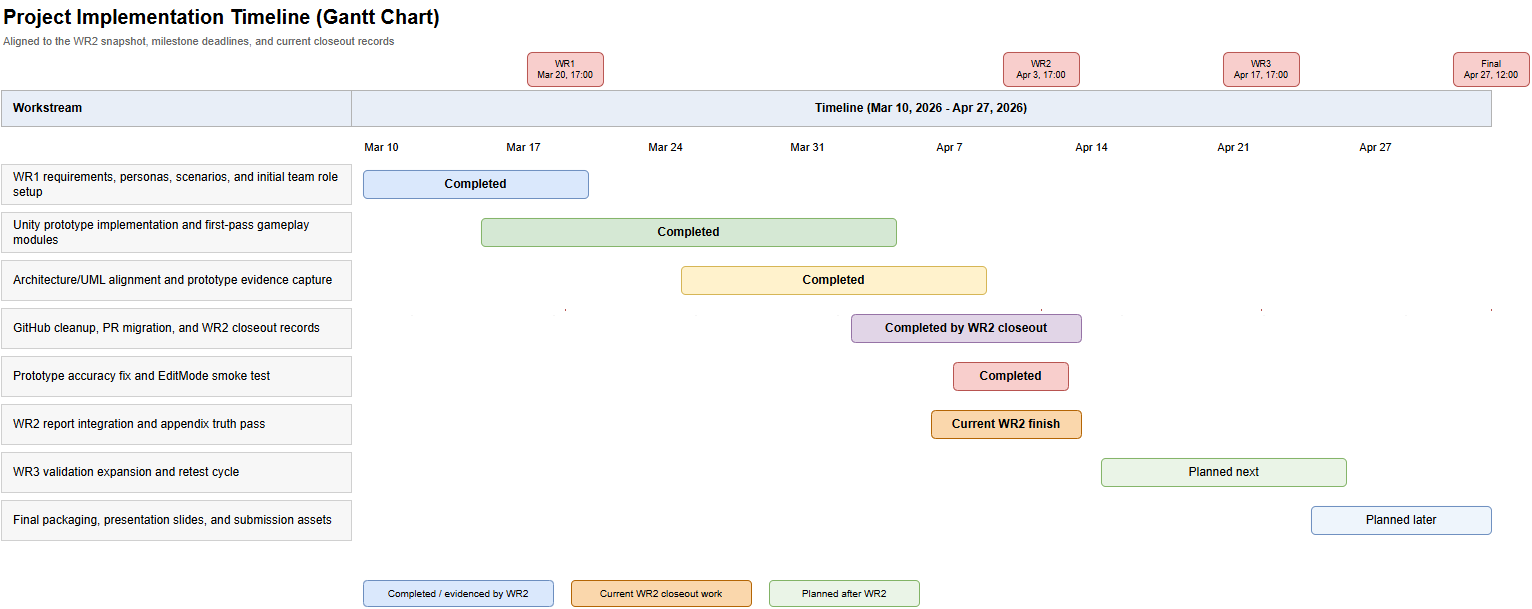
\includegraphics[width=\textwidth]{media/project-implementation-gantt.png}
\caption{Implementation timeline aligned to coursework milestones and the current WR2 closeout snapshot}
\label{fig:implementation-gantt}
\end{figure}

Figure~\ref{fig:implementation-gantt} summarises the timeline from the WR1 foundation through the current WR2 closeout and the planned WR3/final-report stages. The chart separates work already completed in WR2 from work scheduled after the WR2 deadline.

\section{Future Plan}

The next stage connects directly to WR3 and the final report:

\begin{itemize}
\item strengthen battle-end presentation beyond the current top-bar/log feedback and tighten enemy-turn emphasis;
\item improve onboarding cues for first-time interaction with the board and card selection flow;
\item supplement the now-active GitHub PR history with any stronger task-board captures or confirmed attendance evidence the team can still recover;
\item convert the current validation notes into a fuller WR3 testing pack with test cases, bug tracking, and retest records;
\item expand the current automated coverage beyond battle-end behaviour into stable rule-heavy systems such as grid range checks and card resolution rules.
\end{itemize}

In short, WR2 has produced a stable prototype foundation and a clearer list of follow-up work for WR3.
